%!TEX program = xelatex
\documentclass[a4paper]{article}
\usepackage{graphicx}
\usepackage{xcolor}
\usepackage{titlesec, titletoc} %设置标题格式
\usepackage{xeCJK}
\usepackage{fontspec} 
\usepackage{geometry}
\usepackage{fancyhdr}
\usepackage{mdframed}
\usepackage{listings}
\usepackage{amsmath,amssymb}
\usepackage{multirow}
\usepackage{float}
\usepackage{booktabs}
\usepackage{url}
\usepackage{hyperref}
\usepackage{array}
\usepackage[toc,page,title,titletoc,header]{appendix} 
\usepackage{enumerate}
\usepackage{subfig}
\usepackage{natbib}

\bibliographystyle{plain}

% \renewcommand{\thefigure}{\thesection-\arabic{figure}}

\linespread{1.3}

\definecolor{codegreen}{rgb}{0,0.6,0}
\definecolor{codegray}{rgb}{0.5,0.5,0.5}
\definecolor{codepurple}{rgb}{0.58,0,0.82}
\definecolor{backcolour}{rgb}{0.95,0.95,0.92}
\definecolor{codeblack}{rgb}{255,255,255}

\lstdefinestyle{mystyle}{
	backgroundcolor=\color{backcolour},   
	commentstyle=\color{codegreen},
	% keywordstyle=\color{magenta},
	keywordstyle=\color{blue!70},
	numberstyle=\tiny\color{codegray},
	stringstyle=\color{codepurple},
	basicstyle=\footnotesize,
	breakatwhitespace=false,         
	breaklines=true,                 
	captionpos=b,                    
	keepspaces=true,                 
	numbers=left,                    
	numbersep=5pt,                  
	showspaces=false,                
	showstringspaces=false,
	showtabs=false,                  
	tabsize=4,
}
\lstset{style=mystyle}

\geometry{left=2.5cm,right=2.5cm,top=2.5cm,bottom=2.5cm}

% \renewcommand{\thefootnote}{\fnsymbol{footnote}}

\pagestyle{fancy}
\definecolor{dhscodebg}{rgb}{0.85,0.85,0.85}
\newcommand{\HUGE}{\fontsize{29pt}{29pt}\selectfont}

\setmainfont[Mapping=tex-text]{STSONG.TTF}
\lhead{Matlab高级编程与工程应用}
\chead{图像处理大作业实验报告}
\rhead{王禹\ 2014011241 }
\cfoot{\thepage}
\begin{document}
	\pagenumbering{gobble}	
	\begin{titlepage}
		\phantom{Start!}
		\vspace{5cm}
		\begin{center}
			{ \HUGE \bfseries  Matlab高级编程与工程应用}\\[0.4cm]
			{ \HUGE \bfseries  图像处理大作业实验报告}\\[0.4cm]
		\end{center}
		\begin{flushright}
			\vfill
			{
				\newcommand{\pillar}{ {\Huge \phantom{A}} }
				\large
				\begin{tabular}{lc}
					\pillar 姓名 & 王禹 \\
					\pillar 学号 & 2014011241\\
					\pillar 班级 & 无48\\
					\pillar 日期 & 二〇一六年\ 八月\ 二十五日 \\
				\end{tabular}
			}
		\end{flushright}
	\end{titlepage}
	\renewcommand{\contentsname}{目录}
	\tableofcontents
	\newpage
	\pagenumbering{arabic}
	\section{原创性声明}
	本实验完全采用原创设计代码,仅在自主设计JPEG信息隐藏的时候,参考了李思涵同学的思想。
	\section{实验目的}
	\begin{itemize}
		\item 了解计算机存储和处理图像的基础知识;
		\item 掌握JPEG标准的基本原理;
		\item 变化域编码和量化的基本思想;
		\item MATLAB处理矩阵和图像的常用命令;
		\item 在变换域进行信息隐藏的方法;
		\item 学习人脸检测的基本方法。
	\end{itemize}
	
	\section{基础知识}
	\subsection{MATLAB提供了图像处理工具箱,请阅读并大致了解这些函数的基本功能}
	\subsection{利用MATLAB提供的Image file I/O函数分别完成以下处理:}
	\subsubsection{以测试图像的中心为圆心,图像的长和宽中较小值的一半为半径画一个红色的圆;}
	
	图像的读写IO主要依靠MATLAB自带的图像处理工具箱的imread和imwrite函数。将图像读入后,彩色图像为三维矩阵,灰度矩阵为二维矩阵。而本实验中,则是直接load已经准备好的.mat文件,获得图像矩阵。彩色图像的前两维分别为高和宽的像素值,第三维按照顺序为RGB,矩阵的值为0~255的RGB三色的亮度值;灰度图像则没有第三维,只有一个灰度亮度值的二维矩阵。第一问直接获得了图像的矩阵后,找到距离中心小于所指定半径的所有点,将其R分量值调为255,G和B分量都调为0,即可得到所需的图像,最终的结果如下图Figure~\ref{fig1:fi1}所示,而代码如Listing~\ref{lst1:lst1}所示。
	
	\begin{figure}[b]
			\centering
			\subfloat[红圆\label{fig1:fi1}]{
				
\includegraphics[width = .35\textwidth]{../source/3.1/a.jpg}
			}
			\hspace{0.75cm}
			\subfloat[棋格\label{fig1:fi2}]{
				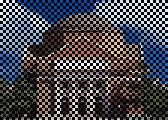
\includegraphics[width = .35\textwidth]{../source/3.1/b.jpg}
			}	
			\caption{题3.1~结果图}
			\label{fig1}
	\end{figure}
	

	\subsubsection{将测试图像涂成国际象棋状的“黑白格”的样子,其中“黑”即为黑色,“白”则意味着保留原图。}
	对于分割为棋盘,为了判断是涂黑还是保持原样,只需判断所要处理的格子的横纵坐标序列数之和的奇偶性即可。结果图见Figure~\ref{fig1:fi2},具体代码见Listing~\ref{lst1:lst2}。
	
	\lstinputlisting[language=Matlab,caption=画红色圆代码,label=lst1:lst1,frame=shadowbox,
	backgroundcolor=\color{white}, rulesepcolor=\color{red!10!green!10!blue!10},,xleftmargin=2em,xrightmargin=2em, aboveskip=1em]{../source/3.1/a.m} 
	
	\lstinputlisting[language=Matlab,caption=涂棋格代码,label=lst1:lst2,frame=shadowbox,
	backgroundcolor=\color{white}, rulesepcolor=\color{red!10!green!10!blue!10},,xleftmargin=2em,xrightmargin=2em, aboveskip=1em]{../source/3.1/b.m} 	
	
	
	\section{图像压缩编码}
	\subsection{图像的预处理是将每个像素灰度值减去128,这个步骤是否可以在变换域进行?} 
	由于变换域的第一个分量便是直流分量,因此这个步骤可以在变换域进行。块是$8 \times 8$ 的像素块,他的DC分量基底为$\frac{1}{8}$,因此将DCT变换后的直流分量减去128即可得到预处理图像。具体代码见Listing~\ref{lst2:lst1}。
	
	根据结果来看,结果相差为$10^{-13}$数量级。
	
	\lstinputlisting[language=Matlab,caption=涂棋格代码,label=lst2:lst1,frame=shadowbox,
	backgroundcolor=\color{white}, rulesepcolor=\color{red!10!green!10!blue!10},,xleftmargin=2em,xrightmargin=2em, aboveskip=1em]{../source/3.2/M2_1.m}

	\subsection{请编程实现二维DCT,并和MATLAB自带的库函数dct2比较是否一致。}
	根据实验指导书前述的二维DCT原理,实现DCT的基底矩阵后,利用矩阵相乘的性质取得dct系数。经过对比后,范数相差仅为$10^{-12}$数量级,可能是由计算中的近似而产生的,因此可以认为自行实现的二维DCT变换和自带库函数dct2是一致的。程序代码参见Listing~\ref{lst2:lst2}。
	
	\lstinputlisting[language=Matlab,caption=涂棋格代码,label=lst2:lst2,frame=shadowbox,
	backgroundcolor=\color{white}, rulesepcolor=\color{red!10!green!10!blue!10},,xleftmargin=2em,xrightmargin=2em, aboveskip=1em]{../source/3.2/M2_2.m}
		
	
	\subsection{如果将DCT系数中右侧四列的系数全部置零,逆变换后图像会发生什么变化?选取一块图像证明你的结论。如果左边四列置零呢?}
	
	\begin{figure}[h]
		\centering
		\subfloat[二维DCT变换基底图像\label{fig2:fi1}\citep{wiki2016wiki}]{
				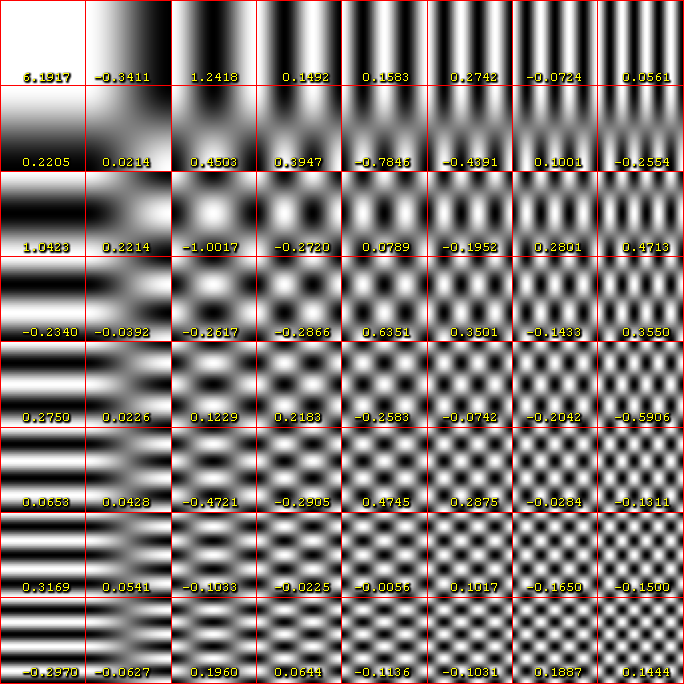
\includegraphics[width = .23\textwidth]{Dct-table.png}	
		}
		\hspace{0.3cm}
		\subfloat[原始图像(左)、右边四列置零(中)、左边四列置零(右)\label{fig2:fi2}]{
			
\includegraphics[width = .23\textwidth]{../source/3.2/origin.jpg}
			\hspace{0.05cm}					
			
\includegraphics[width = .23\textwidth]{../source/3.2/rightzero.jpg}
			\hspace{0.05cm}
			
\includegraphics[width = .23\textwidth]{../source/3.2/leftzero.jpg}
		}	
		\caption{题4.3~结果图}
		\label{fig2}
	\end{figure}
	从Figure~\ref{fig2:fi1} \citep{wiki2016wiki}中可以看出dct系数右侧四列基底在横向上都有高频变化,而左边四列在横向上有低频变化。因此当右侧四列置零时,图像中的横向高频分量丢失,反之当左侧四列置零时,图像中横向低频分量丢失。
	
	测试结果如图Figure~\ref{fig2:fi2}所示。由于我所选择的图片在横向上没有高频变化,主要集中在低频变化上。因此右侧四列原本的值即较小,置零后对图片没有较大的影响,而左侧四列置零后,对图片的影响较大。如结果图所示,左侧四列置零后,整个图片都是黑蒙蒙的一片。
	
	具体代码如Listing~\ref{lst2:lst3}所示。
	
	\lstinputlisting[language=Matlab,caption=涂棋格代码,label=lst2:lst3,frame=shadowbox,
	backgroundcolor=\color{white}, rulesepcolor=\color{red!10!green!10!blue!10},,xleftmargin=2em,xrightmargin=2em, aboveskip=1em]{../source/3.2/M2_3.m}
	
	\subsection{若对DCT系数分别转置、旋转90度和旋转180度操作(rot90),逆变换后恢复的图像有何变化?}
	
		\begin{figure}[b]
			\centering
			\subfloat[原始图像\label{fig3:fi1}]{
				
\includegraphics[width = .12\textwidth]{../source/3.2/origin_rot.jpg}
			}
			\hspace{0.75cm}
			\subfloat[转置图像\label{fig3:fi2}]{
				
\includegraphics[width = .12\textwidth]{../source/3.2/transpose.jpg}
			}
			\hspace{0.75cm}
			\subfloat[旋转$90^\circ$ \label{fig3:fi3}]{
				
\includegraphics[width = .12\textwidth]{../source/3.2/rightrot90.jpg}
			}
			\hspace{0.75cm}
			\subfloat[旋转$180^\circ$ \label{fig3:fi4}]{
				
\includegraphics[width = .12\textwidth]{../source/3.2/rightrot180.jpg}
			}				
			\caption{题4.4~结果图}
			\label{fig3}
		\end{figure}
	若对DCT系数进行转置,则横纵分量的系数发生互换,因此恢复出来的原图像发生了转置。
	
	若对DCT系数逆时针旋转$90^\circ$,则大部分能量集中到左下角。而左下角系数代表的是横向低频变化、纵向高频变化,因此恢复出来的图像应当在横向上是低频变化,而纵向上呈现量化高频变化。
	
	若对DCT系数逆时针旋转$180^\circ$,则大部分能量集中到右下角。而右下角系数代表的横向纵向都是高频变化,因此恢复出来的在横纵向上都有量化高频变化。
	
	最终恢复出来的结果如图Figure~\ref{fig3}所示,与理论匹配。具体的代码如Listing~\ref{lst2:lst4}所示。
	
	\lstinputlisting[language=Matlab,caption=涂棋格代码,label=lst2:lst4,frame=shadowbox,
	backgroundcolor=\color{white}, rulesepcolor=\color{red!10!green!10!blue!10},,xleftmargin=2em,xrightmargin=2em, aboveskip=1em]{../source/3.2/M2_4.m}
	
	\subsection{如果认为差分编码是一个系统,请绘出这个系统的频率响应,说明他是怎样的滤波器。DC系统先进行差分编码在进行熵编码,说明他是一个怎样的系统。}
	
	不考虑初值,差分方程为:
	\begin{center}
		$ \hat{c}_{D}(n) = c_{D}(n-1) - c_{D}(n) $
	\end{center}
	
	即$ A = [1], B = [-1\ 1] $,直接使用MATLAB的freqz函数即可画出频率响应,即Figure~\ref{fig4}。
	代码如Listing~\ref{lst2:lst5}所示。
	
	\begin{figure}[H]
		\centering
		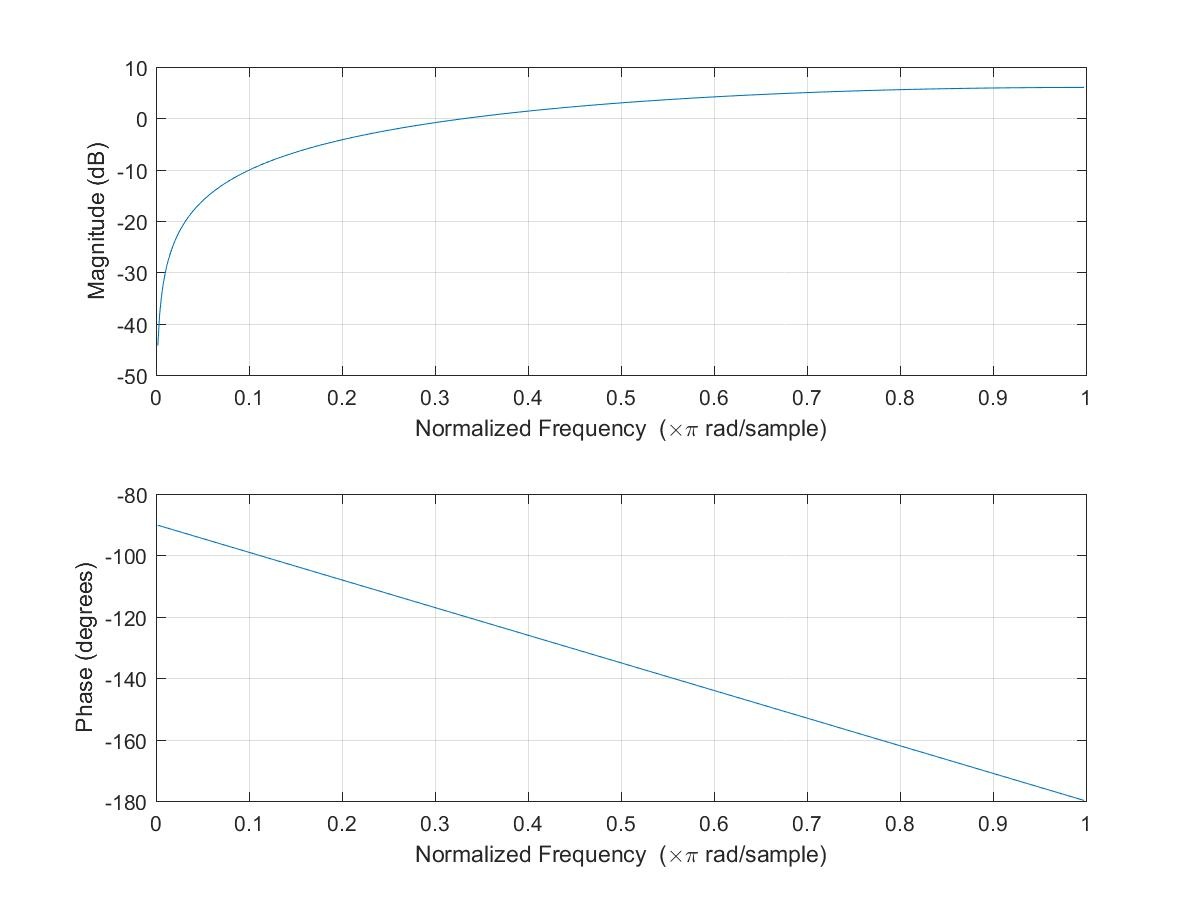
\includegraphics[width = .65\textwidth]{../source/3.2/frequency_plot.jpg}
		\caption{频率响应}
		\label{fig4}
	\end{figure}
	
	
	\lstinputlisting[language=Matlab,caption=频率响应代码,label=lst2:lst5,frame=shadowbox,
	backgroundcolor=\color{white}, rulesepcolor=\color{red!10!green!10!blue!10},,xleftmargin=2em,xrightmargin=2em, aboveskip=1em]{../source/3.2/M2_5.m}
	
	因此这是一个高通系统。而DC系统先进行差分编码再进行熵编码说明DC系统的低频分量较多,故经过系统后能量会有很大的衰减,从而实现信息压缩。
	
	\subsection{DC预测误差取值和Category值有何关系?如何利用预测误差计算出其Category?}
	
	从表中不难观察出,DC误差的取值所对应的二进制长度即为Category值。用数学表达式表述为:
	\begin{center}
		$ Category = ceil(log_2(|value| + 1)) $
	\end{center}
	
	\subsection{你知道哪些实现Zig-Zag扫描方法?请利用MATLAB强大功能设计一种最佳方法。}
	
	共有两种方法:
	
	第一种方法是知己将表格制作好,然后直接存在MATLAB中。这种方法需要自己实现编写好已知位数的zig-zag顺序列表,较为笨拙,但是实际程序运行时效率较高。本实验中采用的便是这种方法,但是效率较高。具体代码见Listing~\ref{lst2:lst6}。
	
	\lstinputlisting[language=Matlab,caption=zigzag代码,label=lst2:lst6,frame=shadowbox,
	backgroundcolor=\color{white}, rulesepcolor=\color{red!10!green!10!blue!10},,xleftmargin=2em,xrightmargin=2em, aboveskip=1em]{../source/3.2/zigzag.m}
	
	第二种方法是设置较为复杂的边界条件,每次碰到边界则横移转向/数移转向。这样的方法可以方便的生成任意尺寸的zig-zag序列,但是每次生成一次序列所需的时间较长,效率较低。因此我采用的是前一种zig-zag生产方法。
	
	\subsection{对测试图像分块、DCT和量化,将量化后的系数写成矩阵的形式,其中每一列为一个块的DCT系数Zig-Zag扫描后形成的列矢量,第一行为各个块儿的DC系数。}
	
	有了上述的Zig-Zag列后,可以很容易的将DCT系数按顺序变为一个列向量,然后放入矩阵中,代码清单Listing~\ref{lst2:lst7}中的代码可以实现这个目的。
	
	\lstinputlisting[language=Matlab,caption=coef矩阵代码,label=lst2:lst7,frame=shadowbox,
	backgroundcolor=\color{white}, rulesepcolor=\color{red!10!green!10!blue!10},,xleftmargin=2em,xrightmargin=2em, aboveskip=1em]{../source/3.2/M2_8.m}
	
	\subsection{请实现JPEG编码,输出为DC系数的码流、AC系数的码流、图像高度和图像宽度,将这四个变量写入jpegcodes.mat文件}
	
	为实现JPEG编码需要按照分块、DCT、量化、熵编码的顺序进行编码。
	
	\subsubsection{分块、DCT、量化}
	为了实现分块,需要原图像的宽和高的像素数目都为8的倍数。本大作业使用的hall\_gray的宽高都恰为8的倍数,若宽高不为高的倍数时,将其扩展到离他最近的8的倍数的宽高。新增的像素点用与其相邻的左侧的像素点或上侧的像素点填充。
	
	获得新的图像后,便可以进行$8 \times 8$的分块了与DCT变换了。修改图片像素尺寸的代码见Listing~\ref{lst2:lst7} 10-20行。
	
	而获得了$8 \times 8$的分块后便可以直接进行DCT变换。为了实现量化,使用的是./的运算,之后使用zigzag(8)的序列,将其放入矩阵中。这部分代码见Listing~\ref{lst2:lst7} 20-26行。
	
	\subsubsection{DC熵编码}
	
	DC系数即为coef矩阵的第一行。首先我们要对这一行系数做一个差分处理,从而消除低频分量达到压缩的目的。差分部分的代码见Listing~\ref{lst2:lst7} 30-36行。差分处理完成后将根据误差的值计算其对应的Category编号,见Listing~\ref{lst2:lst7} 第38行。而第40行对应的是根据Category编号查找Huffman编码,第41-51行对应的是将差分值的二进制编码与Huffman编码编入码流的过程。其中若差分值为负数,则将其1-补码编入码流中。
	
	\subsubsection{AC熵编码}
	
	DC系数处理完成后,我们继续处理AC熵编码。依次从矩阵中按列取出处理AC系数。	我的处理方法为找到这列系数中的非零值的位置,根据这些位置可以计算出他们前面分别有几个零。若是零的个数多余15个,则插入ZRL,并将计数器中的零的个数减十六,直到计数器中零的个数不大于15(Listing~\ref{lst2:lst7} 66-69行),
	在按照run/size查找Huffman码(Listing~\ref{lst2:lst7} 74行)。再对amp进行二进制编码便一并加入到码流中。查找方法与编码方法与DC编码一致,将所有非零值处理完成后,插入结束码(Listing~\ref{lst2:lst7} 79行)便可结束这一列的AC编码,加载下一列进行处理。
	
	\lstinputlisting[language=Matlab,caption=JPEG编码代码,label=lst2:lst7,frame=shadowbox,
	backgroundcolor=\color{white}, rulesepcolor=\color{red!10!green!10!blue!10},,xleftmargin=2em,xrightmargin=2em, aboveskip=1em]{../source/3.2/M2_9.m}
	
	\subsection{计算压缩比}
	
	计算压缩比时,需要注意将hall\_gray矩阵数据的uint8格式转为二进制长度,即8位之后在进行压缩比的比较。计算代码与结果见Listing~\ref{lst2:lst8}。
		\lstinputlisting[language=Matlab,caption=计算压缩比代码,label=lst2:lst8,frame=shadowbox,
		backgroundcolor=\color{white}, rulesepcolor=\color{red!10!green!10!blue!10},,xleftmargin=2em,xrightmargin=2em, aboveskip=1em]{../source/3.2/M2_10.m}
	
	\subsection{请实现JPEG解码,输入是你生成的jpegcodes.mat文件。分别用客观(PSNR)和主观方法评价编解码效果如何。}
	
	为了实现JPEG解码,我们需要定位每一个Huffman码的位置。由于不论是AC编码的Huffman编码还是DC编码的Huffman编码,每个Huffman编码都不是其他码的前缀码,因此可以用逐位比较,若是不相同,则直至
	
		\lstinputlisting[language=Matlab,caption=JPEG解码代码,label=lst2:lst9,frame=shadowbox,
		backgroundcolor=\color{white}, rulesepcolor=\color{red!10!green!10!blue!10},,xleftmargin=2em,xrightmargin=2em, aboveskip=1em]{../source/3.2/M2_11.m}
	
	\subsection{将量化步长减小为原来一半,重做编解码。同标准量化步长的情况比较压缩比和图像质量。}
	
		\lstinputlisting[language=Matlab,caption=半量化步长代码,label=lst2:lst10,frame=shadowbox,
		backgroundcolor=\color{white}, rulesepcolor=\color{red!10!green!10!blue!10},,xleftmargin=2em,xrightmargin=2em, aboveskip=1em]{../source/3.2/M2_12.m}
	
	\subsection{看电视时偶尔能看到美丽的雪花图像(见snow.mat),请对其编解码。和测试图像的压缩比和图像质量进行比较,并解释比较结果。}
	
		\lstinputlisting[language=Matlab,caption=雪花编解码代码,label=lst2:lst11,frame=shadowbox,
		backgroundcolor=\color{white}, rulesepcolor=\color{red!10!green!10!blue!10},,xleftmargin=2em,xrightmargin=2em, aboveskip=1em]{../source/3.2/M2_13.m}
	
	\section{信息隐藏}
	
	\subsection{实现本章介绍的空域隐藏方法和提取方法。验证其抗JPEG编码能力。}
	
	asdasd
	
	ALU部分没有经过硬件调试,由于是组合逻辑电路,仿真通过后,便不会产生较大的硬件错误。本部分是一次编写代码便成功通过,且直接嵌入到处理器中进行使用,故本部分无硬件调试过程。
	
	\subsection{依次实现本章介绍的三种变换域信息隐藏方法和提取方法,分析嵌密方法的隐蔽性以及嵌密后JPEG图像的质量变化和压缩比变化}
	
	MIPS单周期处理器在最开始用Vivado进行综合与实现时,总是显示不能满足时序要求。我刚开始不太明白如何处理这一错误,仍然直接将bit文件烧录进FPGA中,结果是CPU不能正常的工作。之后了解到,我们的FPGA的硬件性能有限,不能够直接接入100M的时钟晶振作为单周期处理器的主频工作。在将100M的晶振经过二分频得到的50M时钟接入后,Vivado便能够正常的进行综合与仿真而不再报错了。由于最终验收时,不考虑单周期处理器的最高主频,因此也没有对单周期处理器的主频最高性能进行测试。
	
	单周期处理器另一个调试的问题在控制模块的编写上。由于控制模块所控制的信号太多,信号名称的大小写最开始在各个模块中没能匹配,导致硬件实现出错。在后续的调试中,发现了这个问题所在,然后将其修复。
	
	其他的模块没有太多的问题需要硬件调试。
	
	\subsection{请设计实现新的隐藏算法并分析其优缺点}
	
	流水线的硬件调试给予我们的最大启示是,verilog语言对每个模块都有固定的写法需要遵守,尤其是逻辑判断。
	具体情况是:单个条件若是一位信号则直接用该信号(或取反),若是多位信号则用==或!=目标值;条件之间的运算用按位或、与。
	流水线硬件调试一开始到处报错,与ModelSim调试结果大相径庭。按照上述原则修改之后便一次性通过了。
	
	
	\section{人脸识别}
	
	\subsection{所给资料Faces目录下包含从网络中截取的28张人脸,试以其作为样本训练人脸标准v}
	\subsubsection{样本人脸大小不一致,是否需要首先将图像调整为相同大小}
	
	asdasd
	
	\subsubsection{假设L = 3,4,5,所得的三个v之间有什么关系?}
	
	asdasd
	
	\subsection{设计一种从任意大小的图片中检测任意多张人脸的算法并编程实现(输出图像在判定为人脸的位置加上红色的方框)。随意选取一张多人的照片,对程序进行测试。尝试L分别取不同的值,评价检测结果的区别。}
	
	asdasd
	
	\subsection{对上述图像分别进行如下处理后}
	\subsubsection{顺时针旋转90度}
	
	asdasd
	
	\subsubsection{保持高度不变,宽度变为原来的2倍}
	
	asdasd
	
	\subsubsection{适当改变颜色}
	
	asdasd
	
	
	\subsection{如果可以重新选择人脸样本的训练标准,你觉得应该如何选取?}
	
	asdasd

	\section{实验总结}
	以下为我组三名同学的实验总结:\\
	
	
	通过本次实验,我将在数字逻辑与处理器基础理论课上学习到的MIPS周期处理器理论,在FPGA上用硬件将其实现。我在小组实现CPU中,负责的是ALU和单周期MIPS的编写。
	
	对于具体的编写实现,ALU部分的编写方式和理论课有所不同。在理论课上,我并没有将ALU分为四个部分分别实现,而是将整体进行编写。而实验指导书要求将ALU分四个部分。在实现层次编写后,我认为这样的编写方式,使得整体的结构更为清晰。而对于四个部分的具体代码,我觉得最有趣的部分应该是比较器的代码。因为比较器内部没有实际的使用比较逻辑判断符,而是直接使用由加法器计算产生的结构进行判断与比较。这是我觉得ALU编写过程中最有趣的部分。
	
	而在单周期处理器的实现中,大部分内容和理论课所讲授的一致。但是外设的编写是一大难点。最开始并没有理解外设的具体实现方法,后来经过慢慢的摸索和理解,了解到外设可以认为是一段新的内存,用以存储和外部部件相关的数据,包括要显示的数据或者是控制状态的数据。通过汇编程序对这部分内存进行访问,从而实现与外设的交互。这样慢慢的理解了外设的地位与RAM是等价的,应当放在与RAM并行的位置进行实现。而单周期的实现中另一大难点在于对于IRQ信号的理解。IRQ信号是由外设模块产生,作用于控制模块,从而使得处理器进入内核态进行处理。这对单周期处理器而言,并没有太大的难点,但对于流水线处理器而言,处理IRQ信号至关重要。
	
	总的而言,本次实验对我来说,收获颇丰,第一次实现了自己编写的CPU,还是一个非常有意义的事。不过想对老师提一点建议,就是CPU性能的衡量标准是\textbf{CPU执行时间}=\textbf{指令数} $\times$ \textbf{CPI} $\times$ \textbf{时钟周期(1/主频)}。因此,并不能单单根据主频来判断CPU的性能,因为不同实现方法,对CPI以及程序的行数的影响也会比较大,应当根据三者的综合来进行判断。

	\renewcommand{\UrlFont}{\small\tt}
	\bibliography{bibfile}

\appendix
	\section{代码清单} \label{app:app1}
	
	根目录:/source
		\begin{enumerate}
		\item /3.1
		\item /3.2
		\end{enumerate}

\end{document}